\documentclass{beamer}
\usepackage{comment}
\usepackage[english]{babel}
\usepackage[utf8]{inputenc}
\usepackage{amsmath, amssymb, amsthm}
\usepackage{cmap}
\usepackage[T1]{fontenc}
\usepackage{array}
\usepackage{multicol}
\usepackage{multirow}
\usepackage{blindtext}
\usepackage{subcaption}
\usepackage{bibentry}
\usepackage{wasysym}
\usepackage{makecell}
\usepackage{marvosym}
%\usepackage{enumitem}
%\definecolor{UBCblue}{rgb}{0.09412, 0.27450, 0.53334}
\definecolor{FMFI}{rgb}{1, 0.5098, 0}
\usetheme{default}
\useinnertheme{circles}
\usecolortheme[named=FMFI]{structure}
\setbeamercolor{block body}{bg=FMFI!10}
\setbeamercolor{block title}{bg=FMFI!30}
\setbeamertemplate{blocks}[rounded][shadow]
\setbeamertemplate{navigation symbols}{}
\setbeamertemplate{itemize item}[default]
\usepackage{tikz}
\usetikzlibrary{shapes.geometric}
\usefonttheme[onlymath]{serif}
% \usetikzlibrary{external}
% \tikzexternalize[prefix=images/]
\newtheorem{conjecture}{Conjecture}
\newtheorem{proposition}{Proposition}
\setbeamertemplate{footline}[frame number]
\usepackage{cite}
\renewcommand*{\citeleft}{\!\!}
\renewcommand*{\citeright}{}
% -------------------
% --- Definicia zakladnych pojmov
% --- Vyplnte podla vasho zadania, rok ma byt rok odovzdania
% -------------------
\def\mfrok{2026}
\def\mfnazov{New approaches to nowhere-zero flow problems}
\def\mftyp{Diploma Thesis}
\def\mfautor{Bc. Lukáš Gáborik}
\def\mfskolitel{Mgr. Jozef Rajník, PhD.}
\def\mfoponent{...}

%ak mate konzultanta, odkomentujte aj jeho meno na titulnom liste
\def\mfkonzultant{tit. Meno Priezvisko, tit. }  

\def\mfmiesto{Bratislava, \mfrok}

% študenti BIN a DAV odkomentujú príslušnú dvojicu riadkov
\def\mfodbor{Computer Science}
\def\program{Computer Science }
% pre BIN:
%\def\mfodbor{Computer Science and Biology} 
%\def\program{ Bioinformatics }
% pre DAV:
% \def\mfodbor{Computer Science and Mathematics} 
% \def\program{Data Science}

% Ak je školiteľ z FMFI, uvádzate katedru školiteľa, zrejme by mala byť aj na zadaní z AIS2
% Ak máte externého školiteľa, uvádzajte Katedru informatiky 
\def\mfpracovisko{Department of Computer Science}


\title{\mfnazov}

\subtitle{Master thesis}

\author
{Lukáš Gáborik}

\institute[]
{
  \begin{figure}
      \centering
      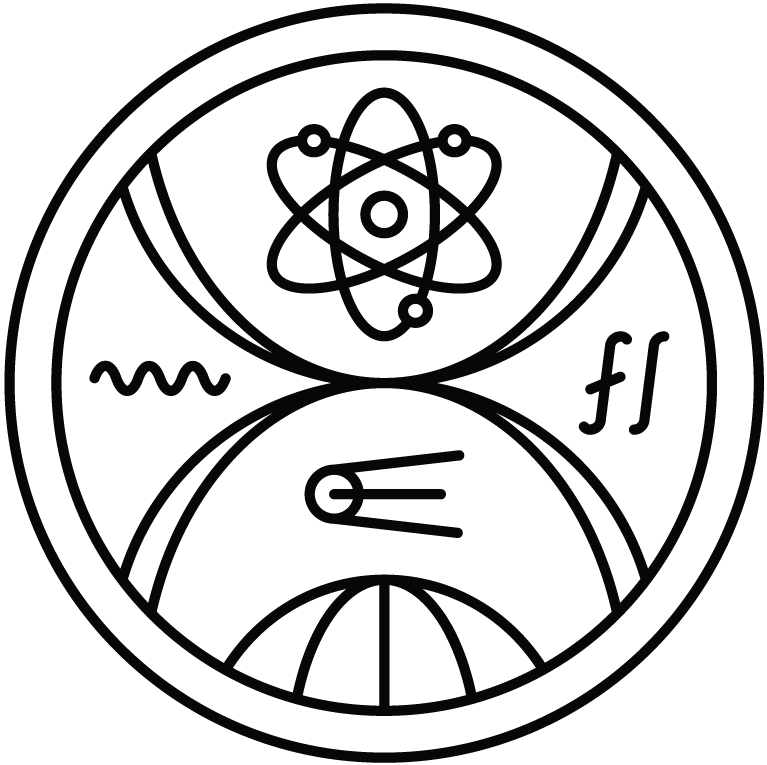
\includegraphics[width=0.15\linewidth]{../logo_FMFI.png}
  \end{figure}
}

\date{21$^\text{st}$ January 2025}

\AtBeginSection[]

\begin{document}

\begin{frame}\titlepage\end{frame}

\begin{frame}{Nowhere-zero $k$-flows}
	\begin{figure}
		\centering
		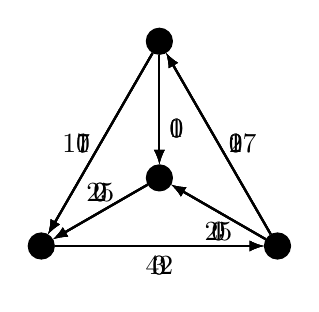
\begin{tikzpicture}[auto,scale=0.5]

	\node (c0) [circle, draw, fill=black] at (0, 0) {};
	\node (c1) [circle, draw, fill=black] at (6, 0) {};
	\node (c2) [circle, draw, fill=black] at (3, 5.2) {};
	\node (c3) [circle, draw, fill=black] at (3, 1.73) {};

	\path<1>
	(c0) edge[-latex, thick] node[below] {$42$} (c1)
	(c1) edge[-latex, thick] node[right] {$17$} (c2)
	(c2) edge[-latex, thick] node[below right] {$0$} (c3)
	(c2) edge[-latex, thick] node[left] {$17$} (c0)
	(c3) edge[-latex, thick] node[above] {$25$} (c0)
	(c1) edge[-latex, thick] node[below] {$25$} (c3);
	
	\path<2>
	(c0) edge[-latex, thick] node[below] {$0$} (c1)
	(c1) edge[-latex, thick] node[right] {$0$} (c2)
	(c2) edge[-latex, thick] node[below right] {$0$} (c3)
	(c2) edge[-latex, thick] node[left] {$0$} (c0)
	(c3) edge[-latex, thick] node[above] {$0$} (c0)
	(c1) edge[-latex, thick] node[below] {$0$} (c3);
	
	\path<3>
	(c0) edge[-latex, thick] node[below] {$3$} (c1)
	(c1) edge[-latex, thick] node[right] {$2$} (c2)
	(c2) edge[-latex, thick] node[below right] {$1$} (c3)
	(c2) edge[-latex, thick] node[left] {$1$} (c0)
	(c3) edge[-latex, thick] node[above] {$2$} (c0)
	(c1) edge[-latex, thick] node[below] {$1$} (c3);

\end{tikzpicture}

		\caption{\only<1>{$43$-flow}\only<2>{$1$-flow}\only<3>{NZ $4$-flow, $\Phi(K_4)=4$}}
	\end{figure}
	\begin{itemize}
		\item<1-> assignment of values $0, 1, 2, \dots, k-1$ to edges
		\item<1-> Kirchoff's law in vertices
		\item<2-> this allowing trivial cases
		\item<2-> restrict zero flow values
		\item<3> graph with NZ $k$-flow has also a NZ $(k+1)$-flow
		\item<3> rate of graph complexity
		\item<3> flow number $\Phi(\Gamma)$ -- minimum
	\end{itemize}
\end{frame}

\begin{frame}{Chebyshev NZ $r$-flows}
	\begin{figure}
		\centering
		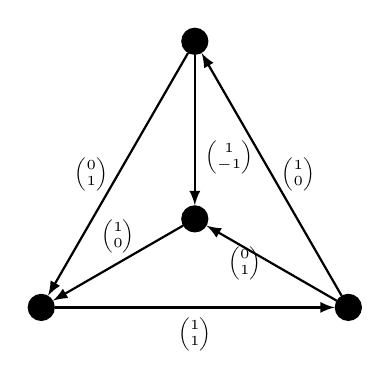
\begin{tikzpicture}[auto,scale=0.65]

	\node (c0) [circle, draw, fill=black] at (0, 0) {};
	\node (c1) [circle, draw, fill=black] at (6, 0) {};
	\node (c2) [circle, draw, fill=black] at (3, 5.2) {};
	\node (c3) [circle, draw, fill=black] at (3, 1.73) {};

	\path
	(c0) edge[-latex, thick] node[below] {\tiny $\begin{pmatrix}1 \\ 1\end{pmatrix}$} (c1)
	(c1) edge[-latex, thick] node[right] {\tiny $\begin{pmatrix}1 \\ 0\end{pmatrix}$} (c2)
	(c2) edge[-latex, thick] node[below right] {\tiny $\begin{pmatrix}1 \\ -1\end{pmatrix}$} (c3)
	(c2) edge[-latex, thick] node[left] {\tiny $\begin{pmatrix}0 \\ 1\end{pmatrix}$} (c0)
	(c3) edge[-latex, thick] node[above] {\tiny $\begin{pmatrix}1 \\ 0\end{pmatrix}$} (c0)
	(c1) edge[-latex, thick] node[left] {\tiny $\begin{pmatrix}0 \\ 1\end{pmatrix}$} (c3);
	
\end{tikzpicture}

		\caption{2D ChNZ $2$-flow, $\Phi_2^\infty(\Gamma)=2$}
	\end{figure}
	\begin{itemize}
		\item generalisation of one-dimensional flows
		\item $\left\|(x_1,x_2)^T\right\|_\infty=\max\{|x_1|, |x_2|\}\in[1, r-1]$
		\item flow number $\Phi_2^\infty(\Gamma)$		
	\end{itemize}
\end{frame}

\begin{frame}{Known bounds}
	\begin{itemize}
		\item generally proved $\Phi(\Gamma)\leq 6$
		\item generally conjectured $\Phi(\Gamma)\leq 5$
		\item for cubic graphs, $3$-colourable iff $\Phi(\Gamma)\leq 4$
		\item generally proved $\Phi_2^\infty(\Gamma)\leq 3$
		\item generally conjectured $\Phi_2^\infty(\Gamma)\leq 5/2$
		\item for cubic graphs, $3$-colourable iff $\Phi_2^\infty(\Gamma)=2$
	\end{itemize}
\end{frame}

\begin{frame}{Sufficient flow-pairs}
	\begin{itemize}
		\item NZ $6$-flow constructed by Seymour from $2$-flow and $3$-flow
		\begin{center}\begin{tabular}{c|c}
			value of $2$-flow & admitted values of $3$-flow\\ \hline
			0 & 1, 2\\
			1 & 0, 1, 2
		\end{tabular}\end{center}
		\item using same flow pair we can construct 2D ChNZ $3$-flow
		\item conjectured $2$-flow and $4$-flow, implying NZ $5$-flow and 2D ChNZ $5/2$-flow
		\begin{center}\begin{tabular}{c|c}
			value of $2$-flow & admitted values of $4$-flow\\ \hline
			0 & 2, 3\\
			1 & 0, 1, 2, 3
		\end{tabular}\end{center}
	\end{itemize}
\end{frame}

\begin{frame}{Seymour's $k$-closures and $k$-bases}
	\begin{figure}
		\centering
		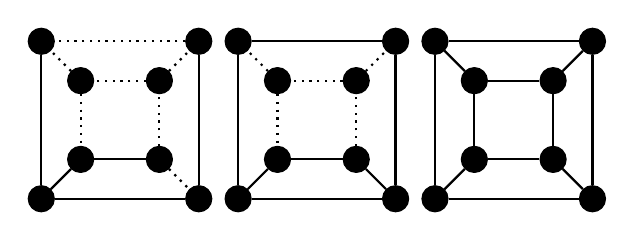
\begin{tikzpicture}[auto,scale=0.5]

	\node (c0) [circle, draw, fill=black] at (0, 0) {};
	\node (c1) [circle, draw, fill=black] at (2, 0) {};
	\node (c2) [circle, draw, fill=black] at (2, 2) {};
	\node (c3) [circle, draw, fill=black] at (0, 2) {};
	\node (c4) [circle, draw, fill=black] at (-1, -1) {};
	\node (c5) [circle, draw, fill=black] at (3, -1) {};
	\node (c6) [circle, draw, fill=black] at (3, 3) {};
	\node (c7) [circle, draw, fill=black] at (-1, 3) {};

	\path[thick]
	(c0) edge (c1)
	(c1) edge[dotted] (c2)
	(c2) edge[dotted] (c3)
	(c3) edge[dotted] (c0)
	(c4) edge (c5)
	(c5) edge (c6)
	(c6) edge[dotted] (c7)
	(c7) edge (c4)
	(c0) edge (c4)
	(c1) edge[dotted] (c5)
	(c2) edge[dotted] (c6)
	(c3) edge[dotted] (c7);
	
	\node (d0) [circle, draw, fill=black] at (5, 0) {};
	\node (d1) [circle, draw, fill=black] at (7, 0) {};
	\node (d2) [circle, draw, fill=black] at (7, 2) {};
	\node (d3) [circle, draw, fill=black] at (5, 2) {};
	\node (d4) [circle, draw, fill=black] at (4, -1) {};
	\node (d5) [circle, draw, fill=black] at (8, -1) {};
	\node (d6) [circle, draw, fill=black] at (8, 3) {};
	\node (d7) [circle, draw, fill=black] at (4, 3) {};

	\path[thick]
	(d0) edge (d1)
	(d1) edge[dotted] (d2)
	(d2) edge[dotted] (d3)
	(d3) edge[dotted] (d0)
	(d4) edge (d5)
	(d5) edge (d6)
	(d6) edge (d7)
	(d7) edge (d4)
	(d0) edge (d4)
	(d1) edge (d5)
	(d2) edge[dotted] (d6)
	(d3) edge[dotted] (d7);
	
	\node (e0) [circle, draw, fill=black] at (10, 0) {};
	\node (e1) [circle, draw, fill=black] at (12, 0) {};
	\node (e2) [circle, draw, fill=black] at (12, 2) {};
	\node (e3) [circle, draw, fill=black] at (10, 2) {};
	\node (e4) [circle, draw, fill=black] at (9, -1) {};
	\node (e5) [circle, draw, fill=black] at (13, -1) {};
	\node (e6) [circle, draw, fill=black] at (13, 3) {};
	\node (e7) [circle, draw, fill=black] at (9, 3) {};

	\path[thick]
	(e0) edge (e1)
	(e1) edge (e2)
	(e2) edge (e3)
	(e3) edge (e0)
	(e4) edge (e5)
	(e5) edge (e6)
	(e6) edge (e7)
	(e7) edge (e4)
	(e0) edge (e4)
	(e1) edge (e5)
	(e2) edge (e6)
	(e3) edge (e7);

\end{tikzpicture}

		\caption{$2$-base of $Y_4$, its $1$-closure and $2$-closure}
	\end{figure}
	\begin{itemize}
		\item $k$-closure -- add a circuit, which has at most $k$ missing edges
		\item $k$-base -- its $k$-closure is the original graph
		\item spanning tree is a $1$-base
	\end{itemize}
\end{frame}

\begin{frame}{Flows and $k$-bases}
	\begin{itemize}
		\item for a $k$-base $X\subseteq E$, there exists a $(k+1)$-flow that is non-zero on $E\setminus X$
		\item ``each'' graph has a $2$-base, that is a ``cycle''
	\end{itemize}
\end{frame}

\begin{frame}{Group connectivity}
	\begin{itemize}
		\item analogue of list colourings
		\item we can deny any flow value for each of the edges
	\end{itemize}
	Forbidding more values
	\begin{itemize}
		\item $k$-base $X\subseteq E$, $n$-flow $\to$ we can forbid \textbf{strictly less than} $n/k$ values for edges from $E\setminus X$
		\item inequality not strict $\Rightarrow$ $2$-flow and $4$-flow with $0,1$ forbidden on $0$ edges of the $2$-flow $\Rightarrow$ conjectures on NZ $5$-flow and ChNZ $2.5$-flow proved
		\item prove for at least some classes of graphs
	\end{itemize}
\end{frame}

\begin{frame}{Lower bound on $\Phi_2^\infty$ for snarks}
	\begin{itemize}
		\item we proved
		\begin{equation*}
			\Phi_2^\infty\geq 2+\left.1\middle/\left\lfloor\frac{n-2}4\right\rfloor\right.
		\end{equation*}
		\item tight for Petersen snarks, Blanuša snarks, but no other equality cases known
		\item can we do better?
	\end{itemize}
\end{frame}

\begin{frame}{Generation of snarks with given girth $g$}
	\begin{itemize}
		\item naive algorithm -- adding $K_2$
		\begin{figure}
			\centering
			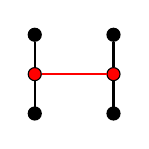
\begin{tikzpicture}[auto,scale=0.5]

	\node (c0) [circle, draw, fill=black, scale=0.5] at (0, 0) {};
	\node (c1) [circle, draw, fill=black, scale=0.5] at (0, 2) {};
	\node (c2) [circle, draw, fill=black, scale=0.5] at (2, 0) {};
	\node (c3) [circle, draw, fill=black, scale=0.5] at (2, 2) {};
	\node (c4) [circle, draw, fill=red, scale=0.5] at (0, 1) {};
	\node (c5) [circle, draw, fill=red, scale=0.5] at (2, 1) {};

	\path[thick]
	(c0) edge (c4)
	(c4) edge (c1)
	(c2) edge (c5)
	(c5) edge (c3)
	(c4) edge[red] (c5);

\end{tikzpicture}

		\end{figure}
		\item last level of generation lasts the most -- try adding tripod instead of last two levels
		\begin{figure}
			\centering
			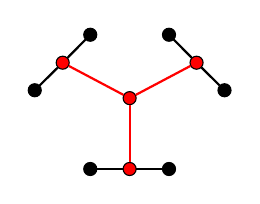
\begin{tikzpicture}[auto,scale=0.5]

	\node (c0) [circle, draw, fill=black, scale=0.5] at (0, 0) {};
	\node (c1) [circle, draw, fill=black, scale=0.5] at (2, 0) {};
	\node (c2) [circle, draw, fill=black, scale=0.5] at (0, 3.41) {};
	\node (c3) [circle, draw, fill=black, scale=0.5] at (-1.41, 2) {};
	\node (c4) [circle, draw, fill=black, scale=0.5] at (2, 3.41) {};
	\node (c5) [circle, draw, fill=black, scale=0.5] at (3.41, 2) {};
	\node (c6) [circle, draw, fill=red, scale=0.5] at (1, 0) {};
	\node (c7) [circle, draw, fill=red, scale=0.5] at (-0.7, 2.7) {};
	\node (c8) [circle, draw, fill=red, scale=0.5] at (2.7, 2.7) {};
	\node (c9) [circle, draw, fill=red, scale=0.5] at (1, 1.8) {};

	\path[thick]
	(c0) edge (c6)
	(c6) edge (c1)
	(c2) edge (c7)
	(c7) edge (c3)
	(c4) edge (c8)
	(c8) edge (c5)
	(c6) edge[red] (c9)
	(c7) edge[red] (c9)
	(c8) edge[red] (c9);

\end{tikzpicture}

		\end{figure}
		\item even better with $6$-vertex subgraph $\mathcal H$
		\begin{figure}
			\centering
			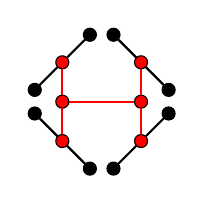
\begin{tikzpicture}[auto,scale=0.5]

	\node (c0) [circle, draw, fill=red, scale=0.5] at (0, 0) {};
	\node (c1) [circle, draw, fill=red, scale=0.5] at (0, 2) {};
	\node (c2) [circle, draw, fill=red, scale=0.5] at (2, 0) {};
	\node (c3) [circle, draw, fill=red, scale=0.5] at (2, 2) {};
	\node (c4) [circle, draw, fill=red, scale=0.5] at (0, 1) {};
	\node (c5) [circle, draw, fill=red, scale=0.5] at (2, 1) {};
	\node (c6) [circle, draw, fill=black, scale=0.5] at (-0.7, 0.7) {};
	\node (c7) [circle, draw, fill=black, scale=0.5] at (0.7, -0.7) {};
	\node (c8) [circle, draw, fill=black, scale=0.5] at (-0.7, 1.3) {};
	\node (c9) [circle, draw, fill=black, scale=0.5] at (0.7, 2.7) {};
	\node (c10) [circle, draw, fill=black, scale=0.5] at (1.3, -0.7) {};
	\node (c11) [circle, draw, fill=black, scale=0.5] at (2.7, 0.7) {};
	\node (c12) [circle, draw, fill=black, scale=0.5] at (1.3, 2.7) {};
	\node (c13) [circle, draw, fill=black, scale=0.5] at (2.7, 1.3) {};

	\path[thick]
	(c0) edge[red] (c4)
	(c4) edge[red] (c1)
	(c2) edge[red] (c5)
	(c5) edge[red] (c3)
	(c4) edge[red] (c5)
	(c6) edge (c0)
	(c0) edge (c7)
	(c8) edge (c1)
	(c1) edge (c9)
	(c10) edge (c2)
	(c2) edge (c11)
	(c12) edge (c3)
	(c3) edge (c13);

\end{tikzpicture}

		\end{figure}
	\end{itemize}
\end{frame}

\begin{frame}{Properties of generation}
	\begin{itemize}
		\item each graph with $g\geq 5$ has a reducible tripod, after reduction, $g'\geq g-1$
		\item each graph with $g\geq 5$ has a reducible $\mathcal H$, after reduction, $g'\geq g-2$
	\end{itemize}
\end{frame}

\begin{frame}{Thank you for your attention!}{Any questions?}
	\begin{figure}
		\centering
		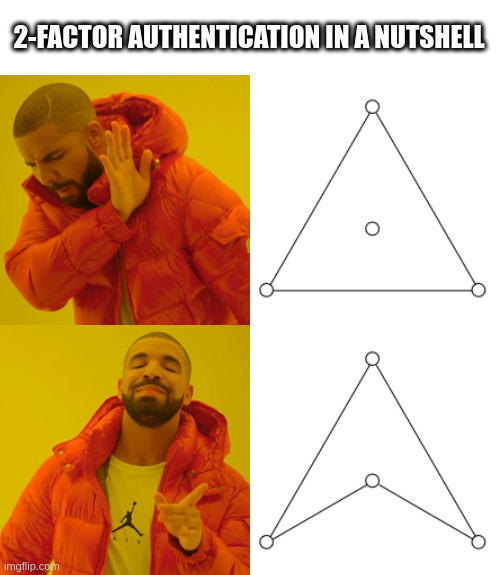
\includegraphics[width=60mm]{2FA_meme.jpg}
	\end{figure}
		
\end{frame}

\end{document}
